\chapter{Encuesta}\label{app1:Encuesta}

\section{Datos Generales}
Estas preguntas contienen las características generales de los participantes, con el propósito de contextualizar los resultados obtenidos.
\begin{figure}[H]
	\centering
	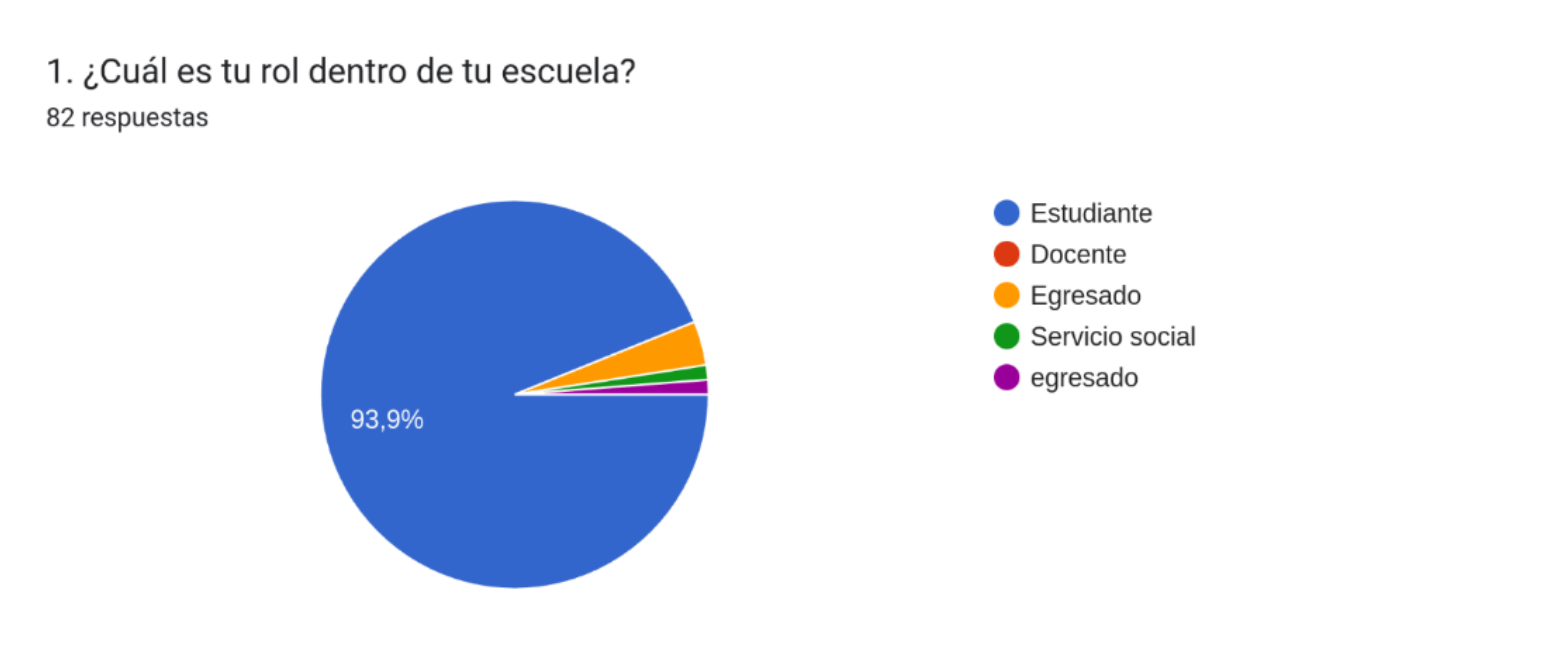
\includegraphics[width=0.9\textwidth]{img/appendixA/1_roles_dentro_de_escuela.png}
	\caption[Roles de los encuestados.]{Roles de los encuestados. \textit{Fuente: Elaboración propia}}
	\label{fig:app1_cantidad_encuestados}  % Etiqueta para la figura
\end{figure}

\begin{figure}[H]
	\centering
	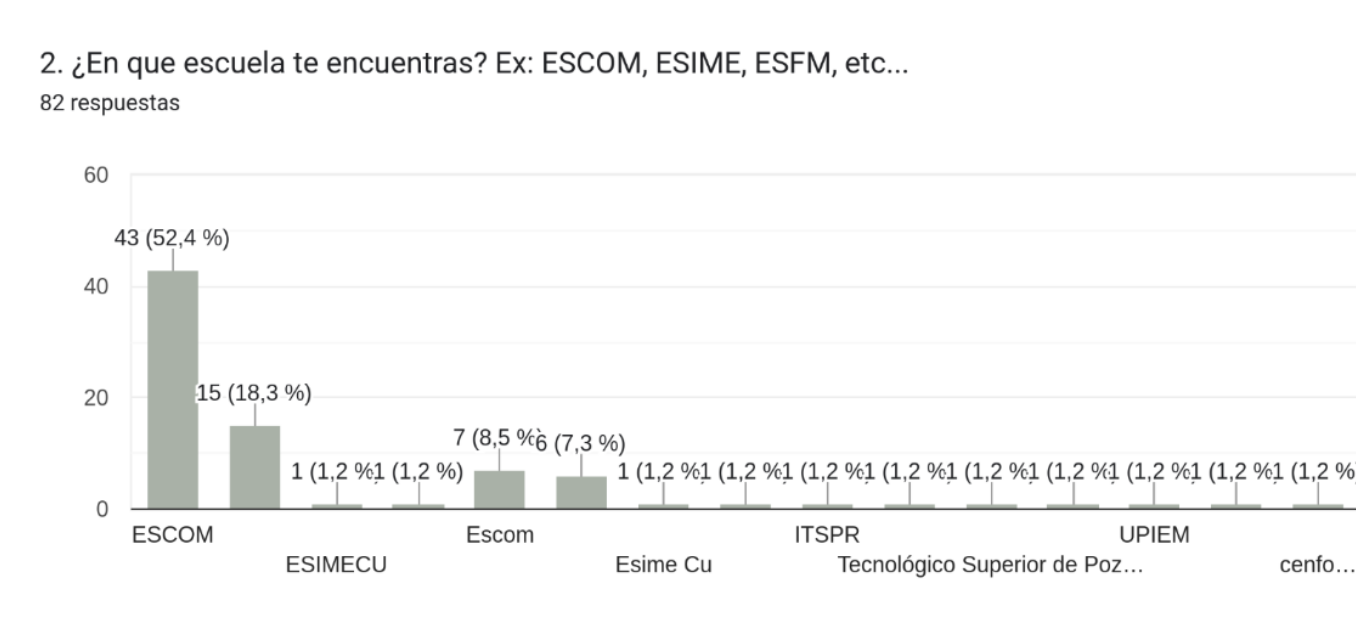
\includegraphics[width=1\textwidth]{img/appendixA/2_escuelas_encuestadas.png}
	\caption[Cantidad de personas encuestadas por escuela]{Cantidad de personas encuestadas por escuela \textit{Fuente: Elaboración propia}}
	\label{fig:app1_escuelas_encuestadas}  % Etiqueta para la figura
\end{figure}

\begin{figure}[H]
	\centering
	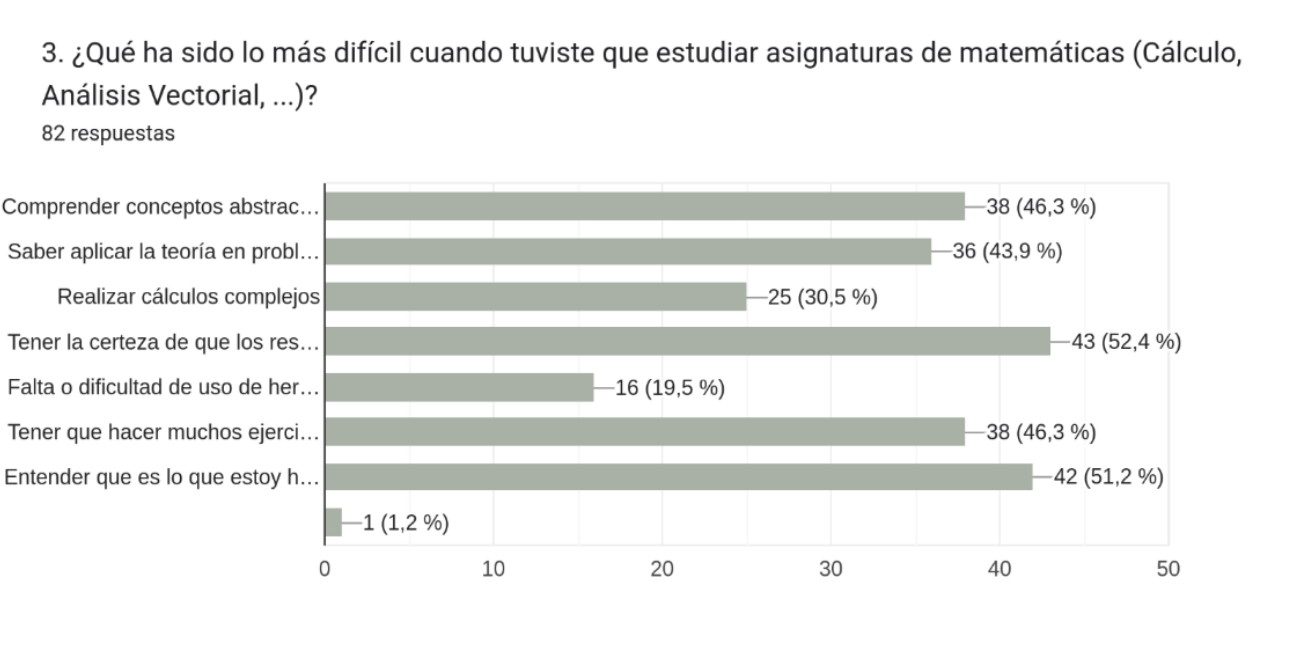
\includegraphics[width=0.9\textwidth]{img/appendixA/3_dificil_en_mates.png}
	\caption[Cantidad de personas encuestadas por escuela]{Cantidad de personas encuestadas por escuela \textit{Fuente: Elaboración propia}}
	\label{fig:app1_dificultad_en_mates}  % Etiqueta para la figura
\end{figure}

\begin{figure}[H]
	\centering
	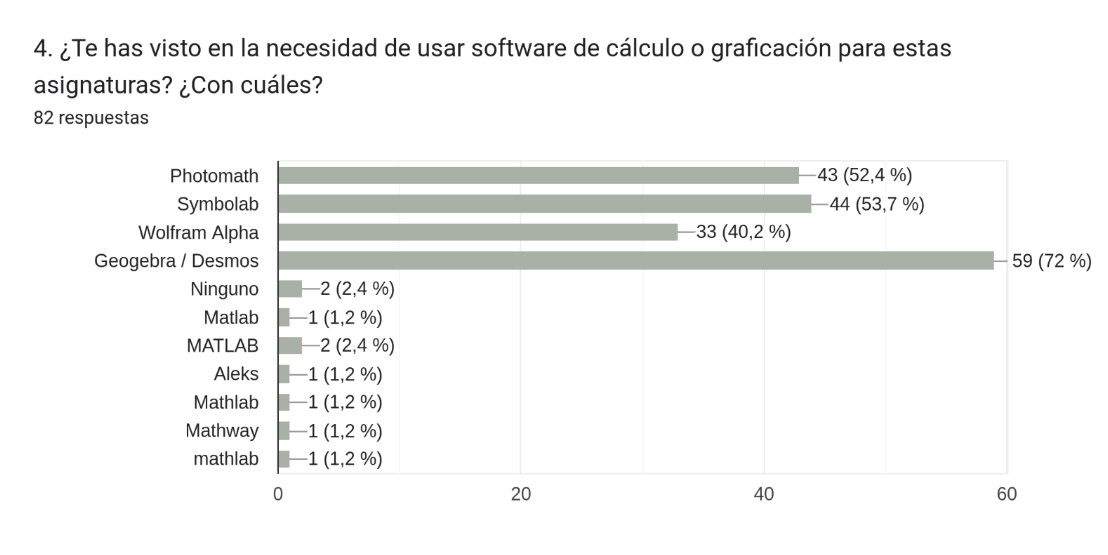
\includegraphics[width=1\textwidth]{img/appendixA/4_software_para_mates.png}
	\caption[Cantidad de personas encuestadas por escuela]{Cantidad de personas encuestadas por escuela \textit{Fuente: Elaboración propia}}
	\label{fig:app1_software_para_mates}  % Etiqueta para la figura
\end{figure}


\begin{figure}[H]
	\centering
	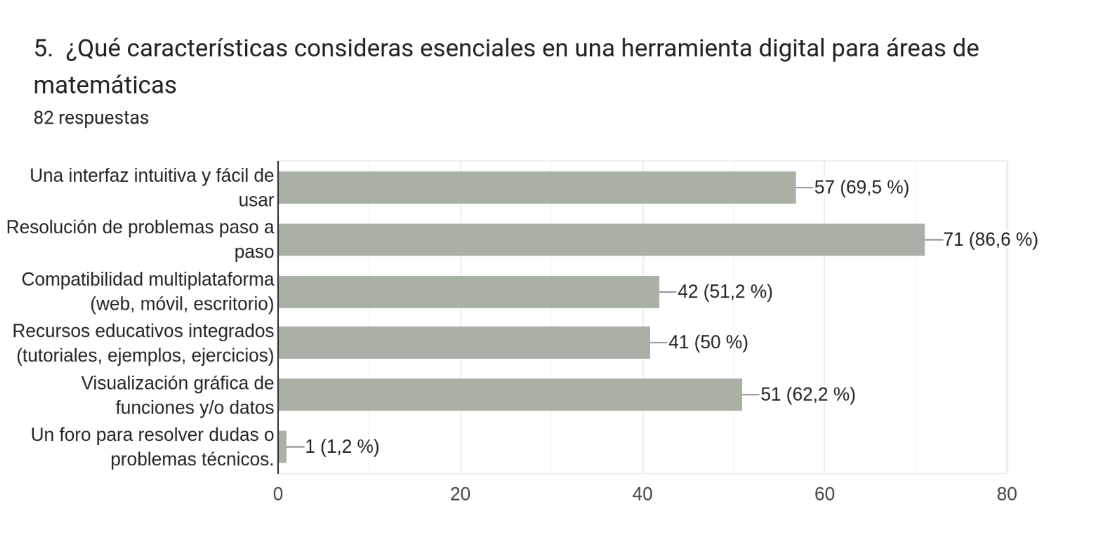
\includegraphics[width=1\textwidth]{img/appendixA/5_caracteristicas_para_app_mates.png}
	\caption[Características que consideran necesarias en recursos digitales para matemáticas.]{Características que consideran necesarias en recursos digitales para matemáticas. \textit{Fuente: Elaboración propia}}
	\label{fig:app1_caracteristicas_para_app_mates}  % Etiqueta para la figura
\end{figure}


\begin{figure}[H]
	\centering
	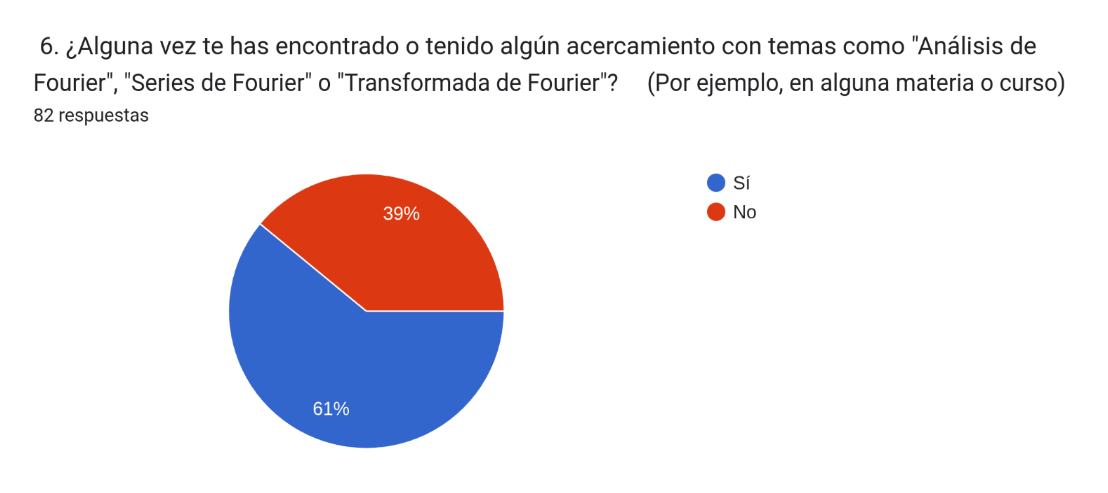
\includegraphics[width=1\textwidth]{img/appendixA/6_Fourier_Filtro.png}
	\caption[Cantidad de alumnos encuestados que han trabajado con problemas de análisis de Fourier.]{Cantidad de alumnos encuestados que han trabajado con problemas de análisis de Fourier.\textit{Fuente: Elaboración propia}}
	\label{fig:app1_Fourier_Filtro}  % Etiqueta para la figura
\end{figure}

\newpage
\section{Participantes con experiencia en Fourier}
Se muestran las respuestas de los participantes que han trabajado previamente con problemas relacionados con series de Fourier, destacando las dificultades encontradas y sus preferencias en herramientas.

\begin{figure}[H]
	\centering
	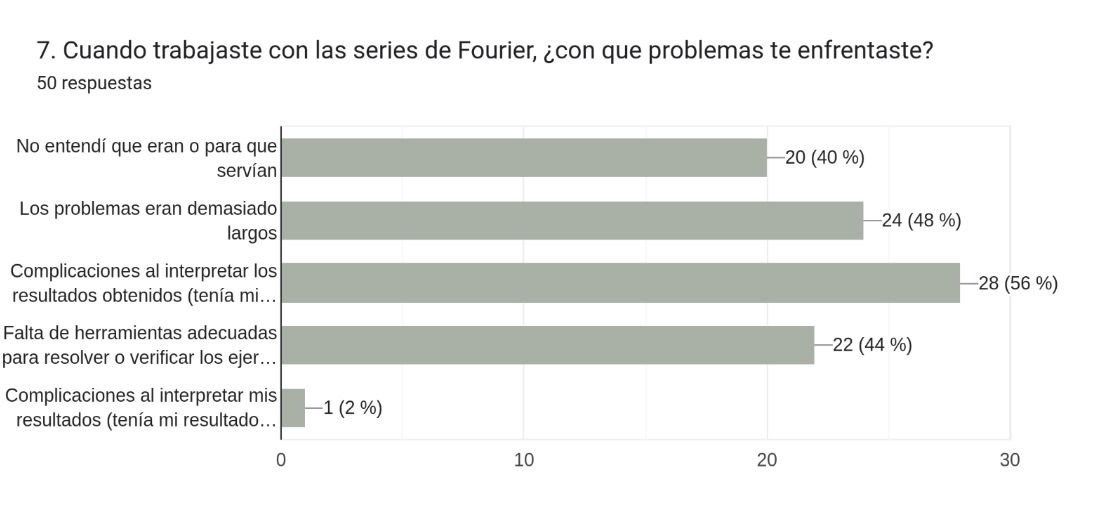
\includegraphics[width=1\textwidth]{img/appendixA/7_problemas_Fourier.png}
	\caption[Problemas que han tenido al trabajar con problemas sobre series de Fourier.]{Problemas que han tenido al trabajar con problemas sobre series de Fourier.\textit{Fuente: Elaboración propia}}
	\label{fig:app1_problemas_Fourier}  % Etiqueta para la figura
\end{figure}

\begin{figure}[H]
	\centering
	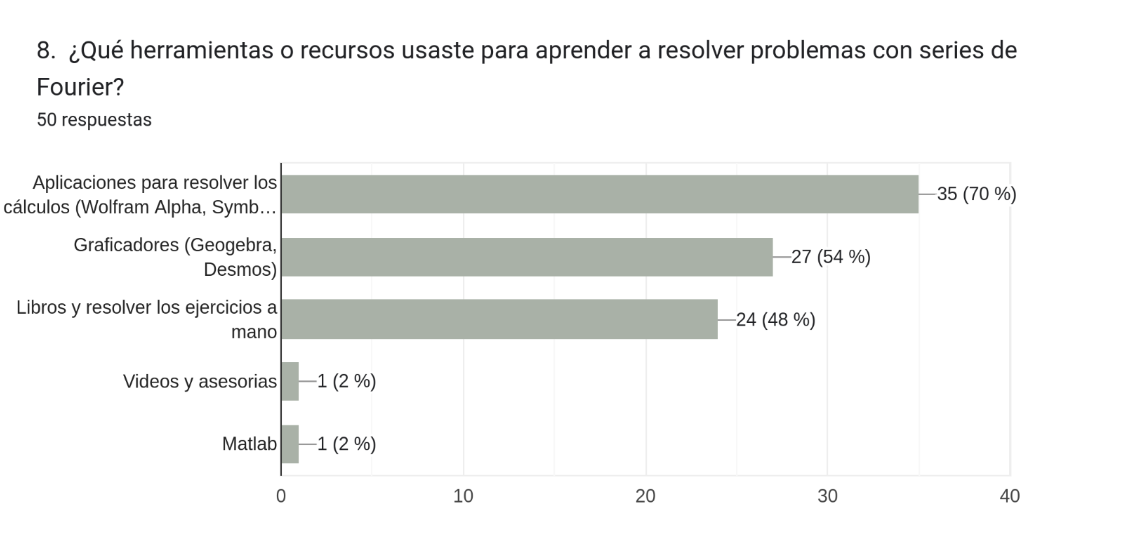
\includegraphics[width=1\textwidth]{img/appendixA/8_herramientas_para_Fourier.png}
	\caption[Problemas que han tenido al trabajar con problemas sobre series de Fourier.]{Problemas que han tenido al trabajar con problemas sobre series de Fourier.\textit{Fuente: Elaboración propia}}
	\label{fig:app1_herramientas_para_Fourier}  % Etiqueta para la figura
\end{figure}

\begin{figure}[H]
	\centering
	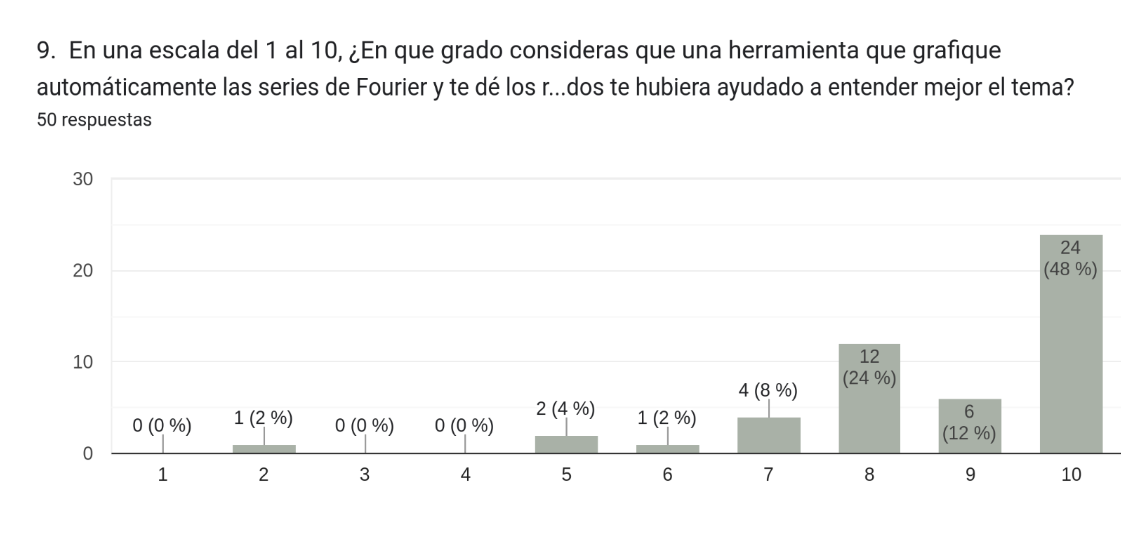
\includegraphics[width=1\textwidth]{img/appendixA/9_grado_de_ayuda_Fourier.png}
	\caption[Problemas que han tenido al trabajar con problemas sobre series de Fourier.]{Problemas que han tenido al trabajar con problemas sobre series de Fourier.\textit{Fuente: Elaboración propia}}
	\label{fig:app1_grado_de_ayuda_Fourier}  % Etiqueta para la figura
\end{figure}

\begin{figure}[H]
	\centering
	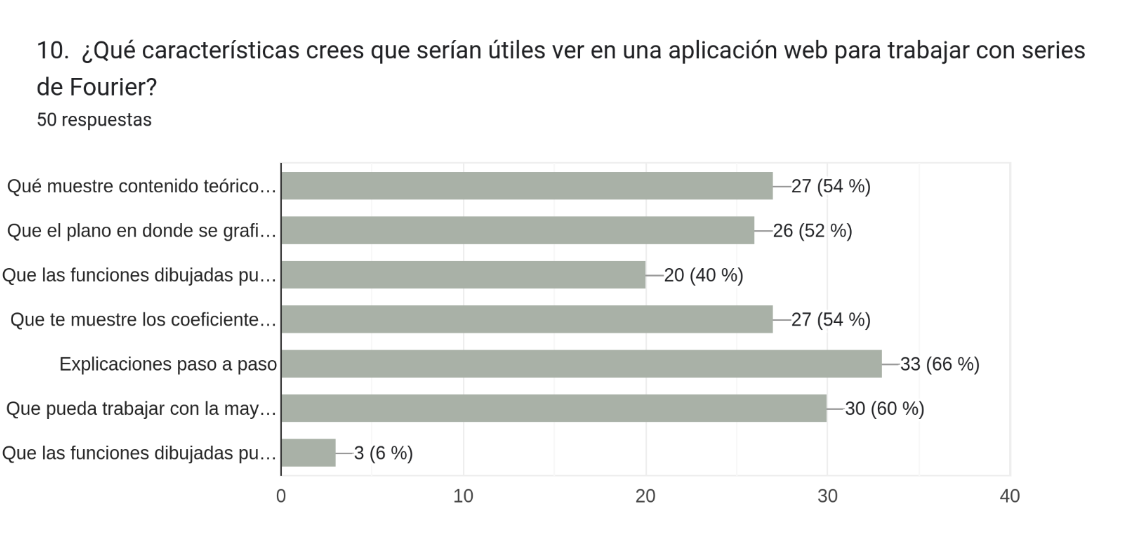
\includegraphics[width=1\textwidth]{img/appendixA/10_cosas_utiles_App_Fourier.png}
	\caption[Problemas que han tenido al trabajar con problemas sobre series de Fourier.]{Problemas que han tenido al trabajar con problemas sobre series de Fourier.\textit{Fuente: Elaboración propia}}
	\label{fig:app1_cosas_utiles_App_Fourier}  % Etiqueta para la figura
\end{figure}

\newpage
\section{Participantes sin experiencia en Fourier}
Se muestran las respuestas de los participantes que no tienen experiencia previa con series de Fourier, incluyendo sus expectativas y preferencias para una herramienta digital que facilite el aprendizaje.

\begin{figure}[H]
	\centering
	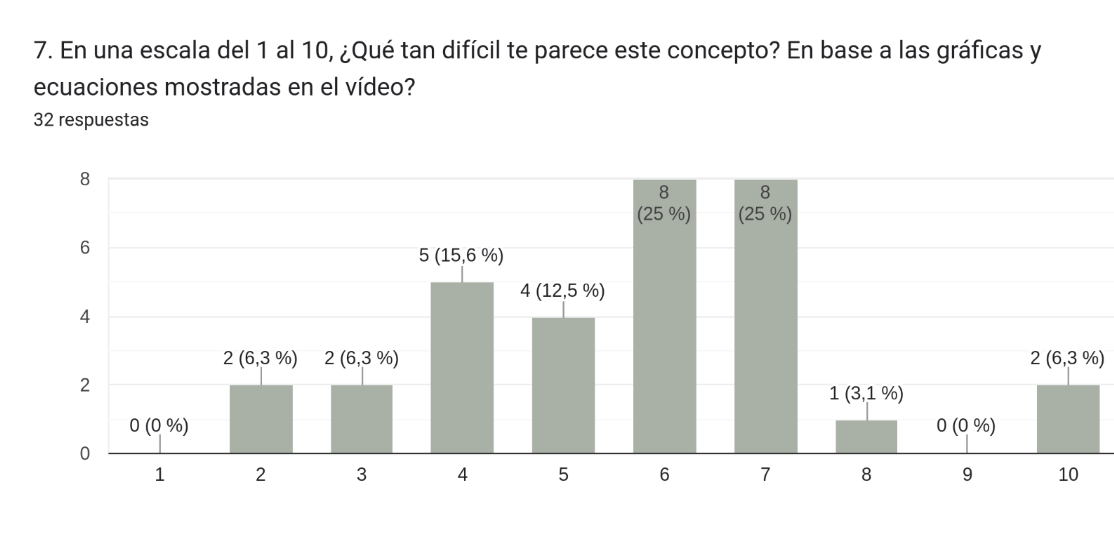
\includegraphics[width=1\textwidth]{img/appendixA/7_dificultad_video_Foruier.png}
	\caption[Problemas que han tenido al trabajar con problemas sobre series de Fourier.]{Problemas que han tenido al trabajar con problemas sobre series de Fourier.\textit{Fuente: Elaboración propia}}
	\label{fig:app1_dificultad_video_Foruier}  % Etiqueta para la figura
\end{figure}

\begin{figure}[H]
	\centering
	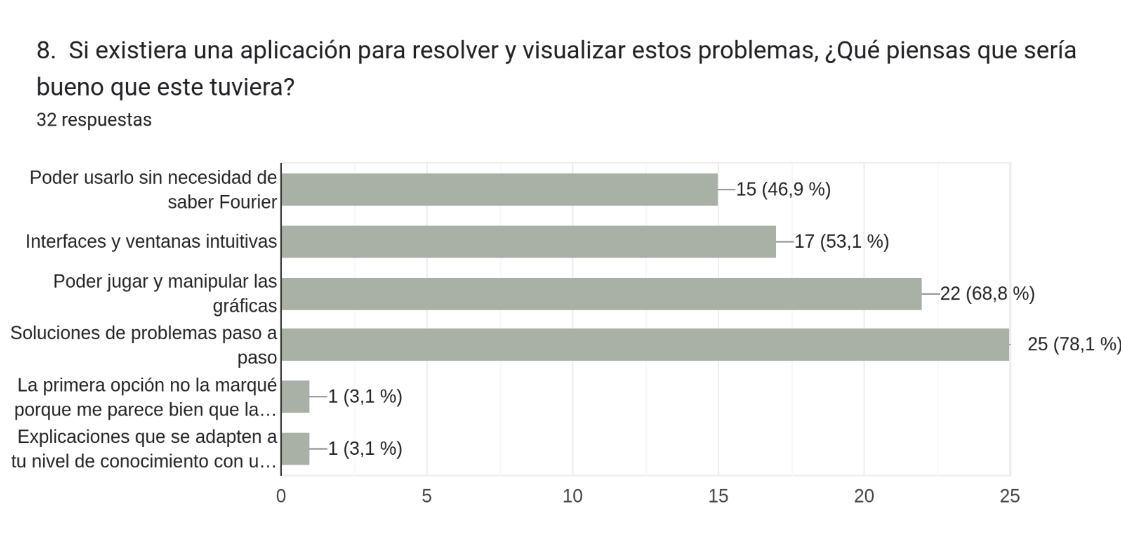
\includegraphics[width=1\textwidth]{img/appendixA/8_cosas_deberie_tener.png}
	\caption[Problemas que han tenido al trabajar con problemas sobre series de Fourier.]{Problemas que han tenido al trabajar con problemas sobre series de Fourier.\textit{Fuente: Elaboración propia}}
	\label{fig:app1_cosas_deberie_tener}  % Etiqueta para la figura
\end{figure}


\newpage
\section{Opinión sobre la utilidad de herramientas digitales}
Se muestran las respuestas de ambos grupos sobre la percepción de la utilidad de una herramienta digital interactiva para resolver y visualizar series de Fourier, así como su valoración de la visualización gráfica.

\begin{figure}[H]
	\centering
	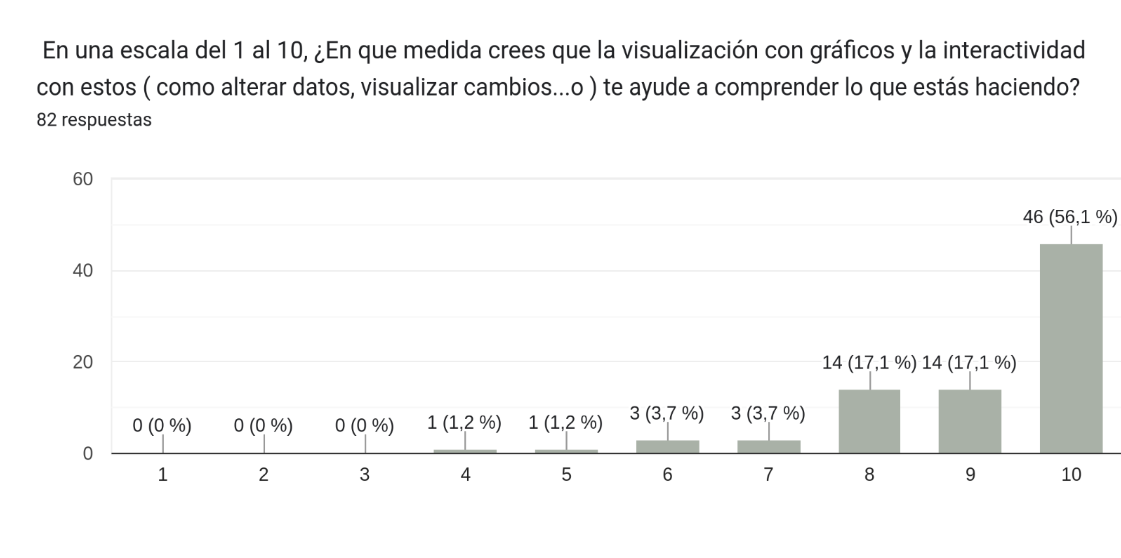
\includegraphics[width=1\textwidth]{img/appendixA/11_importancia_interactividad.png}
	\caption[Problemas que han tenido al trabajar con problemas sobre series de Fourier.]{Problemas que han tenido al trabajar con problemas sobre series de Fourier.\textit{Fuente: Elaboración propia}}
	\label{fig:app1_importancia_interactividad}  % Etiqueta para la figura
\end{figure}

